\section{Stainless Steel}

\subsection{Introduction}

Stainless steel is a relatively new material, having first been developed and refined from the 1800s to the early 1900s, then being defined as a steel with at least 10.5% chromium in 1911\cite{stainlesssteelhistory}.  The addition of Chromium to this level causes the formation of a passive protective layer of Chromium Oxide.  

Iron is alloyed with Chromium, Nickel and Carbon in varying quantities to make Stainless Steel.  Depending on the application, other elements, such as Molybdenum, may be added to enhance the properties of the steel.

\subsection{Grades of Stainless Steel}

While the criteria that qualifies an alloy as Stainless Steel is containing Iron, Carbon and at least 10.5% Chromium, there are many grades that have variety of properties and atomic structures.  The composition influences the structure, resistance to corrosion, yield strength, whether it is magnetic or not, and more.

Both Iron and Chromium are BCC at standard temperatures and pressures, but Nickel is FCC when alloyed it stablizes the austenite phase, FCC, in steel.  Balancing the proportion of these elements changes the phase of the steel, and this may be represented as a Schaeffler diagram or a ternary phase diagram.



\begin{figure}[tbp]
  \begin{center}
    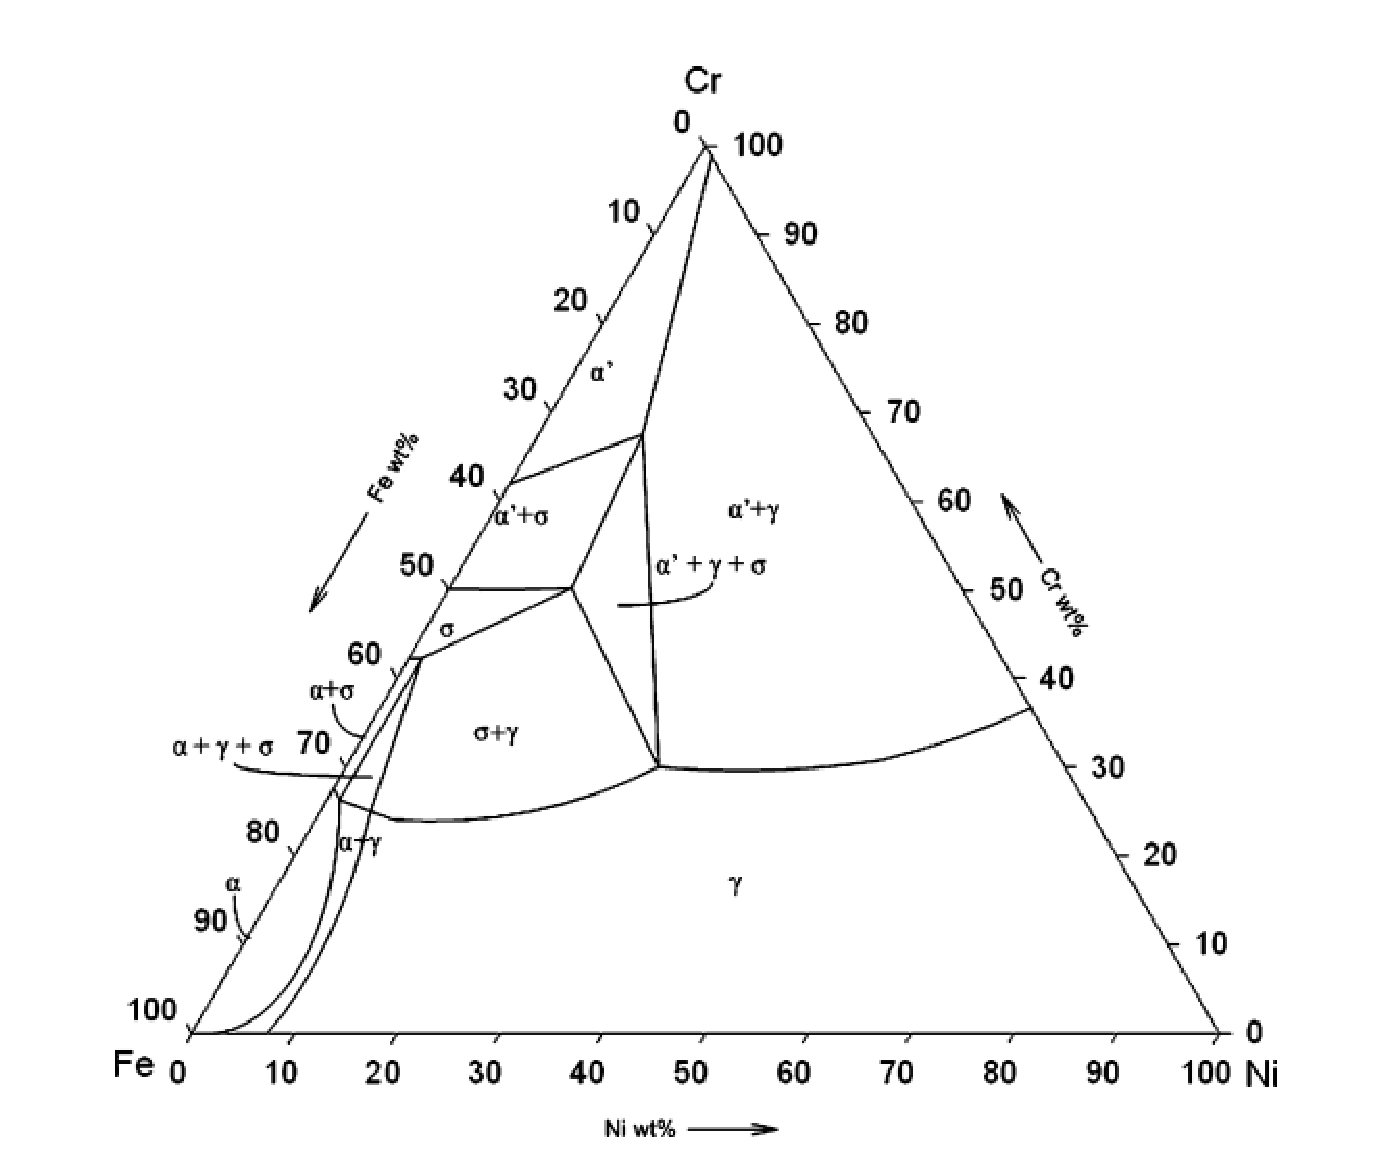
\includegraphics[width=7.0cm]{chapters/background_austenitic_steels_in_nuclear/plots/FeCrNi}
    \caption{Graph caption}
    \label{image:flux1}
  \end{center}
\end{figure}


\begin{figure}[tbp]
  \begin{center}
    \includegraphics[width=7.0cm]{chapters/background_austenitic_steels_in_nuclear/plots/fecrschaeffler.png}
    \caption{Graph caption}
    \label{image:flux1}
  \end{center}
\end{figure}



\subsubsection{Ferritic Stainless Steel}

At room temperatures and pressures, Iron exists in the alpha phase, which is body centered cubic crystal.  It is energetically favourable for the magnetic fields of the iron atoms to align

Ferritic stainless steels have the natural alpha phase crystal structure of pure Iron at room temperature which is bcc.  These steels are magnetic and may be hardened by cold working.  They are less corrosion resistant than austenitic stainless steels.  Two common examples of this grade of steel are ASME (American Society of Mechanical Engineers) codes 405 and 430.


\begin{figure}[ht]
\begin{tikzpicture}[scale=0.40]
\printtikzcrystalbcc{}
\end{tikzpicture} 
\end{figure} 


\subsubsection{Austenitic Stainless Steel}

Austenite is a FCC allotrope of Iron, and austenitic stainless steels are useful in many applications, including a structural material for nuclear plant components, due to their resistance to corrosion.  In addition to 10.5 wt% or more chromium they require an austenite stabilising element such as carbon and/or nickel to be added.

Two examples of such steels are ASME codes 304 and 316.  Both have a high Chromium content, in the region of 18-20%, which is in excess of the minimum passive film requirement of around 10-11%.  The natural structure of such an Fe Cr alloy would be BCC, however 304 and 316 Steels contain Nickel (approximately 8% and 10% respectively) which is an Austenite stabiliser, and this give the FCC structure of the steel.  The 316 grade contains a minimum of 2% Molybdenum to improve its resistance to corrosion.

\begin{figure}[ht]
\begin{tikzpicture}[scale=0.40]
\printtikzcrystalfcc{}
\end{tikzpicture} 
\end{figure} 


\subsubsection{Martensitic Stainless Steel}

Unlike Austenitic and Ferritic, Martensitic stainless steels can be heat treated to harden the steel.  These steels are magnetic and have a FCT crystal structure.  They contain more than 10.5% Chromium and have a much lower Nickel than Austenitic grades, if any.  Two examples of such steels are ASME codes 410 and 431.  

\begin{figure}[ht]
\begin{tikzpicture}[scale=0.40]
\printtikzcrystalfct{}
\end{tikzpicture} 
\end{figure} 


\subsubsection{Property Comparisons}

\begin{table}[h]
\begin{center}
\begin{tabular}{c c c c}
\hline
Grade & Code & Tensile Strength/MPa & Corrosion Potential in Sea Water \\
\hline
Austenitic & 304 & 540-750 & \\
Austenitic & 316 & 520-730 & \\
Ferritic & 405 & 400-600 & \\
Ferritic & 430 & 430-630 & \\
\end{tabular}
\end{center}
\end{table}

















%%The resistance of austenitic stainless steels can be improved further by added other elements, and removing some impurities (or elements found in other standard compositions).  
%%Read: nature of passive films – McBee, Kruger
